\documentclass{article}
\usepackage{preamble}

\title{Unit 7: Stars}
\author{Astronomy\footnote{Access for free at \href{\openstax}{\openstax}} \hspace{0.1ex} at Cypress Springs High School}
\date{Updated on \today}

\numberwithin{equation}{section}
\setcounter{section}{7}
\numberwithin{figure}{section}

\usepackage{fancyhdr}
\pagestyle{fancy}
\renewcommand{\headrulewidth}{0pt}
\renewcommand{\headruleskip}{0mm}
\fancyfoot[C]{Access for free at \href{\openstax}{\openstax} \hfill \thepage}
\fancyhead{}

\makenoidxglossaries

\newglossaryentry{star}{
    name=star,
    description={a massive ball of gas, consisting mostly of hydrogen and helium, that produces its own light across several regions of the electromagnetic spectrum}
}

\newglossaryentry{apparent brightness}{
    name=apparent brightness,
    description={a measure of the amount of light received by Earth from a star or other object—that is, how bright an object appears in the sky, as contrasted with its luminosity}
}

\newglossaryentry{brown dwarf}{
    name=brown dwarf,
    description={an object intermediate in size between a planet and a star; the approximate mass range is from about 1/100 of the mass of the Sun up to the lower mass limit for self-sustaining nuclear reactions, which is about 0.075 the mass of the Sun; brown dwarfs are capable of deuterium fusion, but not hydrogen fusion}
}

\newglossaryentry{luminosity}{
    name=luminosity,
    description={the rate at which a star or other object emits electromagnetic energy into space; the total power output of an object}
}

\newglossaryentry{spectral class}{
    name=spectral class,
    description={(or spectral type) the classification of stars according to their temperatures using the characteristics of their spectra; the types are O, B, A, F, G, K, and M with L, T, and Y added recently for cooler star-like objects that recent survey have revealed}
}

\newglossaryentry{magnitude}{
    name=magnitude,
    description={an older system of measuring the amount of light we receive from a star or other luminous object; the larger the magnitude, the less radiation we receive from the object}
}

\newglossaryentry{binary stars}{
    name=binary stars,
    description={two stars that revolve about each other}
}


\newglossaryentry{H-R diagram}{
    name={H-R diagram},
    description={(Hertzsprung-Russell diagram) a plot of luminosity against surface temperature (or spectral type) for a group of stars}
}

\newglossaryentry{main sequence}{
    name=main sequence,
    description={a sequence of stars on the Hertzsprung–Russell diagram, containing the majority of stars, that runs diagonally from the upper left to the lower right}
}

\newglossaryentry{white dwarf}{
    name=white dwarf,
    description={a low-mass star that has exhausted most or all of its nuclear fuel and has collapsed to a very small size; such a star is near its final state of life}
}

\newglossaryentry{mass-luminosity relation}{
    name=mass-luminosity relation,
    description={the observed relation between the masses and luminosities of many (90\% of all) stars}
}

\newglossaryentry{exoplanet}{
    name=exoplanet,
    description={a planet orbiting a star other than our Sun}
}

\newglossaryentry{giant molecular clouds}{
    name=giant molecular clouds,
    description={large, cold interstellar clouds with diameters of dozens of light-years and typical masses of $10^5$ solar masses; found in the spiral arms of galaxies, these clouds are where stars form}
}

\newglossaryentry{protostar}{
    name=protostar,
    description={a very young star still in the process of formation, before nuclear fusion begins}
}

\newglossaryentry{super-Earth}{
    name=super-Earth,
    description={a planet larger than Earth, generally between 1.4 and 2.8 times the size of our planet}
}

\newglossaryentry{transit}{
    name=transit,
    description={when one astronomical object moves in front of another}
}

\newglossaryentry{mini-Neptune}{
    name=mini-Neptune,
    description={a planet that is intermediate between the largest terrestrial planet in our solar system (Earth) and the smallest jovian planet (Neptune); generally, mini-Neptunes have sizes between 2.8 and 4 times Earth's size}
}

\newglossaryentry{globular cluster}{
    name=globular cluster,
    description={one of about 150 large, spherical star clusters (each with hundreds of thousands of stars) that form a spherical halo around the center of our Galaxy}
}

\newglossaryentry{open cluster}{
    name=open cluster,
    description={a comparatively loose cluster of stars, containing from a few dozen to a few thousand members, located in the spiral arms or disk of our Galaxy; sometimes referred to as a galactic cluster}
}

\newglossaryentry{planetary nebula}{
    name=planetary nebula,
    description={a shell of gas ejected by and expanding away from an extremely hot low-mass star that is nearing the end of its life (the nebulae glow because of the ultra-violet energy of the central star)}
}

\newglossaryentry{nucleosynthesis}{
    name=nucleosynthesis,
    description={the building up of heavy elements from lighter ones by nuclear fusion}
}

\newglossaryentry{main-sequence turnoff}{
    name=main-sequence turnoff,
    description={location in the H-R diagram where stars begin to leave the main sequence}
}

\newglossaryentry{Chandrasekhar limit}{
    name=Chandrasekhar limit,
    description={the upper limit to the mass of a white dwarf (equals 1.4 times the mass of the Sun)}
}

\newglossaryentry{neutron star}{
    name=neutron star,
    description={a compact object of extremely high density composed almost entirely of neutrons}
}

\newglossaryentry{nova}{
    name=nova,
    description={the cataclysmic explosion produced in a binary system, temporarily increasing its luminosity by hundreds to thousands of times}
}

\newglossaryentry{pulsar}{
    name=pulsar,
    description={a variable radio source of small physical size that emits very rapid radio pulses in very regular periods that range from fractions of a second to several seconds; now understood to be a rotating, magnetic neutron star that is energetic enough to produce a detectable beam of radiation and particles}
}

\newglossaryentry{type II supernova}{
    name=type II supernova,
    description={a stellar explosion produced at the endpoint of the evolution of stars whose mass exceeds roughly 10 times the mass of the Sun}
}

\providetoggle{printlines}
\settoggle{printlines}{true}

\providetoggle{printstars}
\settoggle{printstars}{true}

\begin{document}

\maketitle

\subsection{Introduction} \label{wN0Ix8}

In Unit 6, we learned about a few key constellations and the names of some bright stars in them. Recall, for example, the constellations of  Orion the Hunter and Canis Major (the Big Dog):

\begin{center}
\begin{tikzpicture}
\begin{axis}[%
    height=6cm, width=6cm,
    x dir=reverse,
    %axis line style={draw=none},
    ticks=none,
]
\addplot[%
    scatter=true,
    only marks,
    mark=*,
    point meta=explicit symbolic,
    scatter/@pre marker code/.style={/tikz/mark size=\pgfplotspointmeta/4},
    scatter/@post marker code/.style={}
] table [meta index=2] {Unit6_Constellations/Constellations/Orion.dat};

\iftoggle{printstars}{
\node[right=2pt] at (5.24,-8.20) {\footnotesize Rigel};
\node[left=2pt] at (5.92,7.41) {\footnotesize Betelgeuse};
}{}

\iftoggle{printlines}{
\draw
(6.06,19.69) --
(6.20,14.21) --
(6.13,14.77)
(6.20,14.21) --
(6.04,9.65)
(5.91,20.28) --
(6.13,14.77) --
(6.04,9.65) --
(5.92,7.41) --
(5.68,-1.94) --
(5.60,-1.20) --
(5.53,-0.30)
(5.68,-1.94) --
(5.80,-9.67) --
(5.24,-8.20) --
(5.53,-0.30) --
(5.42,6.35) -- % Bellatrix
(5.59,9.93) --
(5.92,7.41)
(5.42,6.35) --
(4.83,6.96) % Tabit
(4.91,10.15) --
(4.84,8.90) --
(4.83,6.96) --% Tabit
(4.85,5.61) --
(4.90,2.44) --
(4.98,1.71)
;

}{}
\end{axis}
\end{tikzpicture}%
\hspace{1cm}
\begin{tikzpicture}
\begin{axis}[%
    height=6cm, width=6cm,
    x dir=reverse,
    %axis line style={draw=none},
    ticks=none,
]
\addplot[%
    scatter=true,
    only marks,
    mark=*,
    point meta=explicit symbolic,
    scatter/@pre marker code/.style={/tikz/mark size=\pgfplotspointmeta/4},
    scatter/@post marker code/.style={}
] table [meta index=2] {Unit6_Constellations/Constellations/CanisMajoris.dat};

\iftoggle{printstars}{
\node[above right=2pt] at (6.75,-16.72) {\footnotesize Sirius};
}{}

\iftoggle{printlines}{
\draw
(7.40,-29.30) -- 
(7.25,-26.77) -- 
(7.14,-26.39) -- % Wezen
(7.03,-27.93) --
(6.98,-28.97) -- 
(6.83,-32.51)
(6.98,-28.97) -- 
(6.34,-30.06)
(7.14,-26.39) -- % Wezen
(7.05,-23.83) --
(6.75,-16.72) -- % Sirius
(6.94,-17.05) -- 
(7.06,-15.63) -- 
(6.90,-12.04) -- 
(6.94,-17.05)
(6.75,-16.72) -- % Sirius
(6.61,-19.26) --
(6.58,-22.96)
(6.38,-17.96) -- 
(6.61,-19.26) --
(6.90,-24.18) -- 
(7.03,-27.93)
;
}{}

\end{axis}
\end{tikzpicture}
\end{center}

But we never addressed the question What is a star? A \gls{star} is a massive ball of gas, consisting mostly of hydrogen and helium, that produces its own light across several regions of the electromagnetic spectrum. The Sun is a star. It's one of about 100 billion ($10^{11}$) stars in the Milky Way Galaxy, and one of about 10 thousand billion billion ($10^{22}$) stars in the entire known universe! Weighing in at \SI{1.99e30}{kg}, the Sun is about 333,000 times more massive than the Earth. It's radius is \SI{6.96e8}{m}, or about 109 times greater than Earth's radius, which implies that it would take 109 side-by-side Earths to span the entire diameter of the Sun. More impressively, the Sun's volume is so large compared to Earth's that you will need 1.3 million Earths to fill the inside of the Sun! Finally, it turns out the Sun is just an average star. There are stars that are way bigger than the Sun.

\begin{center}
\begin{tikzpicture}
\begin{axis}[width=6cm,height=6cm,
    ticks=none,
    xmin=-10,xmax=10,
    ymin=-10,ymax=10,
    clip=false,
    axis line style={draw=none},
]
    \draw (0,0) circle (55pt) node[below=55pt] {Sun};
    \draw[fill=black] (10,-54pt) circle (0.5pt) node[below=1pt] {Earth};
\end{axis}
\end{tikzpicture}
\end{center}

\clearpage
% \begin{multicols}{2}
\subsection*{\ref{wN0Ix8} Exercises}
\textbf{Answer all exercises in complete sentences using correct punctuation.}

\begin{exercise}
    What is a star?
\end{exercise}

\begin{exercise}
    About how many stars are in the Milky Way Galaxy? Write this number in decimal form. For example, $\SI{5.2e4}{}$, which is in scientific notation, is written as 52,400 in decimal form.
\end{exercise}

\begin{exercise}
    Approximately how many stars are in the entire known universe? Again, write this number in decimal form (as opposed to scientific notation).
\end{exercise}

\begin{exercise}
    What is the mass of the Sun in units of kilograms?
\end{exercise}

\begin{exercise}
    Think back to geometry, specifically to circles and spheres. What does radius mean? What is meant by the radius of the Sun? 
\end{exercise}

\begin{exercise}
    What is the radius of the Sun in unit of meters?
\end{exercise}

\begin{exercise}
    Again, think back to geometry. What does the diameter of a circle mean? What is meant by the diameter of the Sun?
\end{exercise}

\begin{exercise}
    If you could align numerous Earths right next to each other in a straight line, how many Earths would it take to span the entire diameter of the Sun?
\end{exercise}

\begin{exercise}
    The volume of the Sun is how many times greater than Earth's volume?
\end{exercise}

\begin{exercise}
    True or False? The Sun is the biggest star in the universe.
\end{exercise}

\begin{exercise}
    In terms of size, how do the stars in the constellations shown at the beginning of the section---Betelgeuse, Rigel, and Sirius---compare to the Sun?
\end{exercise}



% \end{multicols}




\subsection{Luminosity, Color, and Temperature} \label{duzZXq}

The Sun and the stars emit tremendous amounts of energy. Although energy is a difficult concept to define in physics and astronomy, one definition is that energy is ``the amount of stuff that could happen\footnote{Source: \href{https://youtu.be/snj1wBtn6I8}{The Science Asylum}.}.'' For example, lifting a book is something that could (and does) happen when you use your arm strength. Your capacity to lift something comes from the energy in your body that is ultimately stored and transferred from your cells to your muscles. But where did this energy come from? It came from the food you ate, in the form of calories.  Where does your food come from? Plants and animals. Where do cows get their energy? By eating grass. Where does the grass get its energy? Directly from the sun via a process called photosynthesis, in which its plant cells collect and process light energy. Therefore, most things in this world that can and do happen, happen because of energy, and energy comes from the Sun and stars. 

\vspace{1em}

One of the most important characteristic of a star is its \gls{luminosity}---the total amount of energy that a star emits per second. The Sun puts out a tremendous amount of energy every second. (And there are stars far more luminous than the Sun out there.) In physics and chemistry, energy is measured in units of Joules (J). To make the comparison among stars easy, astronomers express the luminosity of other stars in terms of the Sun's luminosity. For example, the luminosity of Sirius is about 25 times that of the Sun. To denote the Sun's luminosity, we use the solar luminosity symbol:

\begin{equation}
    L_{\Sun} = \SI{3.8e26}{W}
\end{equation}

where 1 Watt (W) is is equal to 1 Joule per second. Hence, the luminosity of Sirius can be written as $25\, L_{\Sun}$, which is pronounced ``25 solar luminosities.'' A good analogy for luminosity is a light bulb. A brighter light bulb emits more energy per second than a dimmer light bulb, meaning it has a greater luminosity. 

\vspace{1em}

Stars come in different colors. A star's color is related to its surface temperature. Recall from a previous unit our discussion about the electromagnetic spectrum:
\vspace{1ex}

\begin{mdframed}[backgroundcolor=black!10]
\begin{center}
    Radio \hfill
    Microwave \hfill
    Infrared \hfill
    Visible Light \hfill
    Ultraviolet (UV) \hfill
    X-ray \hfill
    Gamma-ray\\
    \hspace{-10.5ex} (ROY G BIV)\\
    $\leftarrow$ Long wavelength \hfill Short wavelength $\rightarrow$\\
    $\leftarrow$ Low frequency \hfill 
    High Frequency $\rightarrow$\\
    $\leftarrow$ Low energy \hfill High energy $\rightarrow$
\end{center}
\end{mdframed}
\vspace{1ex}

Blue colors dominate the visible light output of very hot stars, with much additional radiation in the ultraviolet. On the other hand, cool stars emit most of their visible light energy at red wavelengths, with more radiation coming off in the infrared. In other words, \textit{hot stars are bluer and cool stars are redder.} (Note: ``Cool'' stars are still very hot in comparison to Earthly temperatures.) The color of a star therefore provides a measure of its true surface temperature. 
%Color does not depend on the distance to the object. This should be familiar to you from everyday experience. The red, yellow, and green colors of a traffic signal, for example, appear the same no matter how far away they are. If we could somehow take a star, observe it, and then move it much farther away, its apparent brightness would change, but this change in brightness is the same for all wavelengths, and so its color would remain the same.

\begin{center}
\begin{tabular}{c|c|c}
    \hline
    \textbf{Star Color} & \textbf{Approximate Temperature} & \textbf{Example} \\
    \hline
     Blue & \SI{25000}{K} (\SI{44500}{\degree\,F}) & Spica\\
     White & \SI{10000}{K} (\SI{17500}{\degree\,F}) & Vega\\
     White/Yellow & \SI{6000}{K} (\SI{10000}{\degree\,F}) & Sun\\
     Orange & \SI{4000}{K} (\SI{6700}{\degree\,F}) & Aldebaran\\
     Red & \SI{3000}{K} (\SI{5000}{\degree\,F}) & Betelgeuse\\
     \hline
\end{tabular}
\end{center}

The hottest stars have temperatures of over \SI{40000}{K} (\SI{71540}{\degree F}), and the coolest stars have temperatures of about \SI{2000}{K} (\SI{3140}{\degree F}). Our Sun's surface temperature is about \SI{6000}{K} (\SI{10000}{\degree F}); its peak wavelength color is a slightly greenish-yellow. In space, the Sun would look white, shining with about equal amounts of reddish and bluish wavelengths of light. It looks somewhat yellow as seen from Earth's surface because our planet's nitrogen molecules scatter some of the shorter (i.e., blue) wavelengths out of the beams of sunlight that reach us, leaving more long wavelength light behind. This also explains why the sky is blue: the blue sky is sunlight scattered by Earth's atmosphere.

%Add to text: Stars don't emit a single wavelength of color: they aren't monochromatic. Rather, they emit a range of color frequencies. For blue stars, the range peaks in and is tilted towards the bluer wavelengths; for red stars, the range tilts toward redder wavelengths. The color of stars that emit approximately equal parts red and blue frequencies is white. 

\subsection*{\ref{duzZXq} Exercises}

\begin{exercise}
    What is luminosity?
\end{exercise}

\begin{exercise}
    Time is measured in units of seconds, minutes, or hours. Mass is measured in pounds or kilograms. Length is measured in meters, inches, or feet. According to the physicists, what are the units of energy?
\end{exercise}

\begin{exercise}
    What are the units of luminosity? What other units are the units of luminosity equivalent to?
\end{exercise}

\begin{exercise}
    What is the luminosity of the Sun (the solar luminosity)? Write this number both in scientific notation and in decimal notation.
\end{exercise}

\begin{exercise}
    The luminosity of a star is like the brightness of which common household item?
\end{exercise}

\begin{exercise}
    Google ``PhET Simulation Energy Forms and Changes'' or \href{https://phet.colorado.edu/en/simulations/energy-forms-and-changes}{click here}. Click the \texttt[red]{Systems} panel and explore the different configurations of energy. What are the different types of energy that exist in the universe?
\end{exercise}

\begin{exercise}
    A star's color is related to which property of the star?
\end{exercise}

\begin{exercise}
    \textit{Review}. What are the 7 regions of the electromagnetic spectrum?
\end{exercise}

\begin{exercise}
    \textit{Review}. What are the 7 colors of the visible portion of the spectrum?
\end{exercise}

\begin{exercise}
    What color are hot stars?
\end{exercise}

\begin{exercise}
    What color are cool stars? (Remember: ``Cool'' stars are still very hot. They're just cool by comparison with the hottest stars.)
\end{exercise}

\begin{exercise}
    What is the temperature, in degrees Fahrenheit, of the hottest stars?
\end{exercise}

\begin{exercise}
    What is the temperature, in degrees Fahrenheit, of the coolest stars?
\end{exercise}

\begin{exercise}
    What is the temperature, in degrees Fahrenheit, of our Sun? Tungsten, the metal with the highest melting point, melts at about \SI{6200}{\degree\,F}, which made it an excellent substance to use in older light bulbs. Can the surface temperature of the Sun melt tungsten?
\end{exercise}

\begin{exercise}
    Why does the Sun look white in space?
\end{exercise}

\begin{exercise}
    Why the Sun look yellow from Earth (especially during sunrise and sunset)?
\end{exercise}

\begin{exercise}
    Why is the sky blue?
\end{exercise}

% \begin{exercise}
%     If you know a star's luminosity and mass, what third property about the star can you determine?
% \end{exercise}

\subsection{The Classification of Spectra of Stars}

Measuring colors is only one way of analyzing starlight. Another way is to use a spectrograph to spread out the light into a spectrum. In 1814, the German physicist Joseph Fraunhofer observed that the spectrum of the Sun shows dark lines crossing a continuous band of colors. In the 1860s, English astronomers \textbf{Sir William Huggins} and \textbf{Lady Margaret Huggins} succeeded in identifying some of the lines in stellar spectra as those of known elements on Earth, showing that the same chemical elements found in the Sun and planets exist in the stars. Since then, astronomers have worked hard to perfect experimental techniques for obtaining and measuring spectra, and they have developed a theoretical understanding of what can be learned from spectra. Today, spectroscopic analysis is one of the cornerstones of astronomical research.

Astronomers use the patterns of lines observed in stellar spectra to sort stars into a spectral class. Because a star's temperature determines which absorption lines are present in its spectrum, these spectral classes are a measure of its surface temperature. There are seven standard spectral classes. From hottest to coldest, these seven spectral classes are designated as follows:
\vspace{-1em}

\begin{align*}
    {\Large \mathrm{O \hspace{2em} 
        B \hspace{2em}
        A \hspace{2em} 
        F \hspace{2em} 
        G \hspace{2em} 
        K \hspace{2em} 
        M}}
\end{align*}

At this point, you may be looking at these letters with wonder and asking yourself why astronomers didn't call the spectral types A, B, C, and so on. You will see, as we tell you the history, that it's an instance where tradition won out over common sense.
\vspace{1em}

In the 1880s, Williamina Fleming devised a system to classify stars based on the strength of hydrogen absorption lines. Spectra with the strongest lines were classified as ``A'' stars, the next strongest ``B,'' and so on down the alphabet to ``O'' stars, in which the hydrogen lines were very weak. But hydrogen lines alone are not a good indicator for classifying stars, since their lines disappear from the visible light spectrum when the stars get too hot or too cold.
\vspace{1em}

In the 1890s, Annie Jump Cannon revised this classification system, focusing on just a few letters from the original system: A, B, F, G, K, M, and O. Instead of starting over, Cannon also rearranged the existing classes---in order of decreasing temperature---into the sequence we have learned: O, B, A, F, G, K, M. Annie Cannon classified around \SI{500000}{} stars over her lifetime, classifying up to three stars per minute by looking at the stellar spectra.
\vspace{1em}

To help astronomers remember this crazy order of letters, Cannon created a mnemonic, ``Oh Be A Fine Girl, Kiss Me.'' (If you prefer, you can easily substitute ``Guy'' for ``Girl.'') Other mnemonics, which we hope will not be relevant for you, include ``Oh Brother, Astronomers Frequently Give Killer Midterms'' and ``Oh Boy, An F Grade Kills Me!''

\begin{exercise}
    Create your own mnemonic for the \textbf{O\,B\,A\,F\,G\,K\,M} classification of stars.
\end{exercise}



% \subsection{A Stellar Census}
% Stars within 21 Light-Years of the Sun:
% \begin{center}
% \begin{tabular}{c|c}
% \hline
% \textbf{Spectral Type} & \textbf{Number of Stars}\\
% \hline
%     A & 2 \\
%     F &	1 \\
%     G & 7 \\
%     K & 17 \\
%     M & 94 \\
%     % White dwarfs	8
%     % Brown dwarfs	33
% \hline
% \end{tabular}
% \end{center}

\clearpage
\begin{mdframed}[backgroundcolor=black!5]
\textbf{Algol the Demon Star and Perseus the Hero}
\vspace{1em}

The name Algol comes from the Arabic Ras al Ghul, meaning ``the demon's head.'' The word ``ghoul'' in English has the same derivation. Many of the bright stars have Arabic names because during the long dark ages in medieval Europe, it was Arabic astronomers who preserved and expanded the Greek and Roman knowledge of the skies. The reference to the demon is part of the ancient Greek legend of the hero Perseus, who is commemorated by the constellation in which we find Algol and whose adventures involve many of the characters associated with the northern constellations.
\vspace{1em}

Perseus was one of the many half-god heroes fathered by Zeus (Jupiter in the Roman version), the king of the gods in Greek mythology. Zeus had a roving eye and was always fathering somebody or other with a human maiden who caught his fancy. (Perseus derives from Per Zeus, meaning ``fathered by Zeus.'') Set adrift with his mother, Dana\"{e}, by an upset stepfather, Perseus grew up on an island in the Aegean Sea. The king there, taking an interest in Perseus' mother, tried to get rid of the young man by assigning him an extremely difficult task.
\vspace{1em}

In a moment of overarching pride, a beautiful young woman named Medusa had compared her golden hair to that of the goddess Athena (Minerva for the Romans). The Greek gods did not take kindly to being compared to mere mortals, and Athena turned Medusa into a gorgon: a hideous, evil creature with writhing snakes for hair and a face that turned anyone who looked at it into stone. Perseus was given the task of slaying this demon, which seemed like a pretty sure way to get him out of the way forever.
\vspace{1em}

But because Perseus had a god for a father, some of the other gods gave him tools for the job, including Athena's reflective shield and the winged sandals of Hermes (Mercury in the Roman story). By flying over her and looking only at her reflection, Perseus was able to cut off Medusa's head without ever looking at her directly. Taking her head, which could still turn onlookers to stone even without being attached to her body, with him, Perseus continued on to other adventures.
\vspace{1em}

He next came to a rocky seashore, where boasting had gotten another family into serious trouble with the gods. Queen Cassiopeia had dared to compare her own beauty to that of the Nereids, sea nymphs who were daughters of Poseidon (Neptune in Roman mythology), the god of the sea. Poseidon was so offended that he created a sea-monster named Cetus to devastate the kingdom. King Cepheus, Cassiopeia's beleaguered husband, consulted the oracle, who told him that he must sacrifice his beautiful daughter Andromeda to the monster.
\vspace{1em}

When Perseus came along and found Andromeda chained to a rock near the sea, awaiting her fate, he rescued her by turning the monster to stone. (Scholars of mythology actually trace the essence of this story back to far-older legends from ancient Mesopotamia, in which the god-hero Marduk vanquishes a monster named Tiamat. Symbolically, a hero like Perseus or Marduk is usually associated with the Sun, the monster with the power of night, and the beautiful maiden with the fragile beauty of dawn, which the Sun releases after its nightly struggle with darkness.)
\vspace{1em}

Many of the characters in these Greek legends can be found as constellations in the sky, not necessarily resembling their namesakes but serving as reminders of the story. For example, vain Cassiopeia is sentenced to be very close to the celestial pole, rotating perpetually around the sky and hanging upside down every winter. The ancients imagined Andromeda still chained to her rock, as it is much easier to see the chain of stars than to recognize the beautiful maiden in this star grouping. Perseus is next to her with the head of Medusa swinging from his belt. Algol represents this gorgon head and has long been associated with evil and bad fortune in such tales. Some commentators have speculated that the star's change in brightness (which can be observed with the unaided eye) may have contributed to its unpleasant reputation, with the ancients regarding such a change as a sort of evil ``wink.''
\end{mdframed}

\subsection*{Exercises}



\begin{exercise} \label{PfKIgU}
    In Arabic, what does \textit{Ras al Ghul} mean?
\end{exercise}

\begin{exercise}
    Draw a character map of the characters in the Perseus stories. Include Perseus, Zeus, Dana\"{e}, Athena, and any other characters included in the story. Draw arrows between characters to show what they did in the story. You may include quick artistic sketches of the characters.
\end{exercise}

\begin{exercise}
    Draw a sketch of Perseus holding Medusa's head. This is often how Perseus is depicted in statues and art. You may need to look up a few examples.
\end{exercise}

\begin{exercise} \label{WOot0c}
    Research the star Algol online. List three things you learned about the star. 
\end{exercise}

\clearpage

\subsection{The Death of Stars: White Dwarfs} \label{yqCTwS}

\begin{mdframed}[backgroundcolor=black!10]
\textbf{Subrahmanyan Chandrasekhar}
\vspace{1ex}

Born in 1910 in Lahore, India, Subrahmanyan Chandrasekhar (known as Chandra to his friends and colleagues) grew up in a home that encouraged scholarship and an interest in science (Figure 23.3). His uncle, C. V. Raman, was a physicist who won the 1930 Nobel Prize. A precocious student, Chandra tried to read as much as he could about the latest ideas in physics and astronomy, although obtaining technical books was not easy in India at the time. He finished college at age 19 and won a scholarship to study in England. It was during the long boat voyage to get to graduate school that he first began doing calculations about the structure of \textbf{white dwarf stars}.
\vspace{1em}

Chandra developed his ideas during and after his studies as a graduate student, showing that white dwarfs with masses greater than 1.4 times the mass of the Sun cannot exist and that the theory predicts the existence of other kinds of stellar corpses. He wrote later that he felt very shy and lonely during this period, isolated from students, afraid to assert himself, and sometimes waiting for hours to speak with some of the famous professors he had read about in India. His calculations soon brought him into conflict with certain distinguished astronomers, including Sir Arthur Eddington, who publicly ridiculed Chandra's ideas. At a number of meetings of astronomers, such leaders in the field as Henry Norris Russell refused to give Chandra the opportunity to defend his ideas, while allowing his more senior critics lots of time to criticize them.
\vspace{1em}

Yet Chandra persevered, writing books and articles elucidating his theories, which turned out not only to be correct, but to lay the foundation for much of our modern understanding of the death of stars. In 1983, he received the Nobel Prize in physics for this early work.
\vspace{1em}

In 1937, Chandra came to the United States and joined the faculty at the University of Chicago, where he remained for the rest of his life. There he devoted himself to research and teaching, making major contributions to many fields of astronomy, from our understanding of the motions of stars through the Galaxy to the behavior of the bizarre objects called black holes (see Black Holes and Curved Spacetime). In 1999, NASA named its sophisticated orbiting X-ray telescope (designed in part to explore such stellar corpses) the Chandra X-ray Observatory.
\vspace{1em}


Chandra spent a great deal of time with his graduate students, supervising the research of more than 50 PhDs during his life. He took his teaching responsibilities very seriously: during the 1940s, while based at the Yerkes Observatory, he willingly drove the more than 100-mile trip to the university each week to teach a class of only a few students.
\vspace{1em}

Chandra also had a deep devotion to music, art, and philosophy, writing articles and books about the relationship between the humanities and science. He once wrote that ``one can learn science the way one enjoys music or art. . . . Heisenberg had a marvelous phrase ‘shuddering before the beautiful’. . . that is the kind of feeling I have.''
\end{mdframed}

The death of a star depends on its mass. Let's define the mass of the Sun as \SI{1}{M_{\odot}} (pronounced ``1 solar mass''). Then we can speak of the masses of other stars in terms of the solar mass. For example, a star with 5 times the mass of the Sun will have a mass of \SI{5}{M_{\odot}}, or 5 solar masses. 
\vspace{1em}

For a star with an initial mass between 0.08 and \SI{10}{M_{\odot}}, the final state at the end of its life will be a white dwarf star. A white dwarf star is a low-mass star that has exhausted most or all of its nuclear fuel and has collapsed to a very small size. Such a star is near its final state of life. For a star with an initial mass between 10 and \SI{40}{M_{\odot}}, the final state at the end of its life will be a supernova explosion that leaves a neutron star. And for stars whose lifetime masses are greater than \SI{40}{M_{\odot}}, their final state will be a supernova explosion that leaves a black hole (the topic of our next unit). 
\vspace{1em}

\begin{exercise} \label{8kn3PP}
    In what year was Chandra born?
\end{exercise}

\begin{exercise}
    What prize did Chadra's uncle recieve in 1930?
\end{exercise}

\begin{exercise}
    At what age did Chandra finish college? Where did he move to?
\end{exercise}

\begin{exercise}
    What type of star did Chadra study?
\end{exercise}

\begin{exercise}
    What NASA observatory was named after Chandra?
\end{exercise}

\begin{exercise}
    What is a white dwarf star?
\end{exercise}

\begin{exercise}
    What is the fate of a star whose mass is between 0.08 and \SI{10}{M_{\odot}}?
\end{exercise}

\begin{exercise}
    What is the fate of a star whose mass is between 10 and \SI{40}{M_{\odot}}?
\end{exercise}

\begin{exercise} \label{P4iquu}
    What is the fate of a star whose mass is greater than \SI{40}{M_{\odot}}?
\end{exercise}

\subsection{Neutron Stars}

Recall that an atom---the smallest and most basic unit of matter---is composed of protons, electrons, and neutrons. The neutron is the subatomic particle that has a neutral charge (i.e., neither positive nor negative electric charge). In our Earthly world, we do not see neutrons by themselves in massive quantities, because they are always found inside the nucleus of atoms. But in strange parts of the universe, they may be found by themselves in huge quantities, in special objects called neutron stars.
\vspace{1em}

After a supernova explosion fades away, all that is left behind is either a neutron star or something even more strange, a black hole. (We will describe the properties of black holes in the next unit). After their supernova explosions, stars with initial masses between 10 and \SI{40}{M_{\odot}} will leave behind a neutron star.
\vspace{1em}

\begin{figure}[h!]
    \centering
    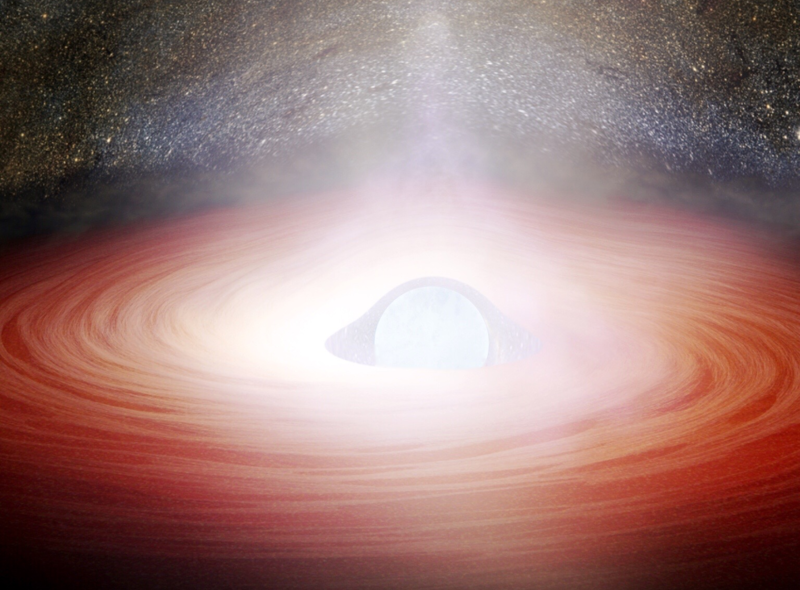
\includegraphics[width=8cm]{Figures/Neutron_Star_simulation.png}
    % \caption{Caption}
    % \label{fig:my_label}
\end{figure}

A \gls{neutron star} is a compact object of extremely high density, composed almost entirely of neutrons. Neutron stars are the densest objects in the universe; the force of gravity at their surface is $10^{11}$ times greater than what we experience at Earth's surface. The interior of a neutron star is composed of about 95\% neutrons, with a small number of protons and electrons mixed in. In effect, a neutron star is a giant atomic nucleus, with a mass about $10^{57}$ times the mass of a proton. Its diameter is more like the size of a small town or an asteroid than a star---about 20 kilometers. Because it is so small, a neutron star probably strikes you as the object least likely to be observed from thousands of light-years away. Yet neutron stars do manage to signal their presence across vast gulfs of space.
\vspace{1em}

\begin{exercise}  \label{SC9S9F}
    What is a neutron star?
\end{exercise}

\begin{exercise}
    What percentage of a neutron star is composed of neutrons?
\end{exercise}

\begin{exercise}
    What is the approximate diameter of a typical neutron star? 
\end{exercise}

\begin{exercise}
    When a \SI{45}{M_{\odot}} star dies in a supernova explosion, will it leave behind a neutron star? Explain. 
\end{exercise}

\begin{exercise} \label{gkUxJg}
    Look up neutron stars on \textit{Wikipedia}. Draw a quick sketch of your favorite example of what a neutron star could look like (we've never seen them up close, as they are really hard to detect).
\end{exercise}


% \gls{spectral class}

% \gls{brown dwarf}

% \gls{binary stars}

% \gls{mass-luminosity relation}

% \gls{H-R diagram}

% \gls{main sequence}

% \gls{white dwarf}

% \gls{giant molecular clouds}

% \gls{protostar}

% \gls{exoplanet} 

% \gls{transit}

% \gls{super-Earth}

% \gls{mini-Neptune}

% \gls{globular cluster}

% \gls{open cluster}

% \gls{main-sequence turnoff}

% \gls{planetary nebula}

% \gls{nucleosynthesis}

% \gls{Chandrasekhar limit}

% \gls{neutron star}

% \gls{type II supernova}

% \gls{pulsar}

% \gls{nova} 


\clearpage
\printnoidxglossaries

\clearpage
\subsection{Additional Resources}

\begin{enumerate}
    \item \textit{Wolfram MathWorld}: ``Radius'' (\href{https://mathworld.wolfram.com/Radius.html}{click here})
    \item \textit{YouTube}: ``Universe Size Comparison 3D'' by \texttt{Harry Evett} (\href{https://youtu.be/i93Z7zljQ7I}{click here}).
    \item \textit{PhET Simulation}: ``Blackbody Spectrum'' (\href{https://phet.colorado.edu/en/simulations/blackbody-spectrum}{click here})
\end{enumerate}

\clearpage
\subsection*{Lesson Plans}


\textbf{Week 3}
\vspace{1ex}

\begin{tabular}{|m{0.25\textwidth}|m{0.7\textwidth}|}
    \hline
    \cellcolor{black!20}\textbf{Date} & \cellcolor{black!20}\textbf{Tuesday, 1/17/2023} \\
    \hline
    Learning Intention (TPO) & Listen to the story of Algol the Demon Star and Perseus the Hero.\\
    \hline 
    Hook/Warm Up/Opening & Create your own mnemonic for the OBAFGKM spectral sequence.\\
    \hline
    Lesson/Learning Activities & Students receive print copy of the Perseus story. As teacher reads, students follow along with their eyes on paper and ears on teacher's voice. \\
    \hline
    Graded Activities & Exercises \ref{PfKIgU} through \ref{WOot0c}\\
    \hline
    Closure & Teacher grades and stamps student work. Students ask finalizing questions.\\
    \hline
    \hline

    \cellcolor{black!20}\textbf{Date} & \cellcolor{black!20}\textbf{Wednesday, 1/18/2023} \\
    \hline
    Learning Intention (TPO) & We will introduce The Death of Stars (Sec.~\ref{yqCTwS}) and define a \gls{white dwarf}.\\
    \hline
    Hook/Warm Up/Opening & Read the brief biography of Subrahmanyan Chandrasekhar, the Nobel laureate and astronomer who made fundamental contributions to the study of white dwarf stars.\\
    \hline
    Lesson/Learning Activities & Whiteboard lecture on white dwarfs. Show diagram of the Sun now vs.~in 8 billions years as a white dwarf star. Show the first few minutes of \href{https://youtu.be/Mj06h8BeeOA?t=39}{this video} to illustrate some fascinating features of white dwarfs. Metaphor: When the Sun becomes a white dwarf, it will be a senile old man/woman assisted by a cane. \\
    \hline
    Graded Activities & Exercises \ref{8kn3PP} through \ref{P4iquu}\\
    \hline
    Closure & Discuss answers to some exercises, and answer student questions.\\
    \hline
    \hline

    \cellcolor{black!20}\textbf{Date} & \cellcolor{black!20}\textbf{Thursday, 1/19/2023} \\
    \hline
    Learning Intention (TPO) & We will learn about \gls{neutron star}s and define a black hole.\\
    \hline
    Hook/Warm Up/Opening & Show the last half of the \href{https://youtu.be/0fKBhvDjuy0?t=331}{Powers of Ten video} so Ss understand how small the neutron is. \\
    \hline
    Lesson/Learning Activities & \textit{Whiteboard lecture}. Define and sketch an atom, including protons, electrons, and neutrons. Under extreme pressure, protons and electrons can fuse to create neutrons. Define neutron star. Neutron star is left behind by stars with masses between 10 and \SI{40}{M_{\odot}} Sketch a neutron star next to city of Houston to compare size. Show this \href{https://youtu.be/udFxKZRyQt4}{Kurzgesagt video} on neutron stars.\\
    \hline
    Graded Activities & Exercises \ref{SC9S9F} through \ref{gkUxJg}. \\
    \hline
    Closure & Discussion about the scientific method. The inside of neutron stars is a deep mystery, as the video explained. How could scientists even begin to understand such mysteries?\\
    \hline
    \hline

    \cellcolor{black!20}\textbf{Date} & \cellcolor{black!20}\textbf{Friday, 1/20/2023} \\
    \hline
    Learning Intention (TPO) & We are reviewing for Tuesday's Test on Unit 7: Stars.\\
    \hline
    Hook/Warm Up/Opening & Watch this \href{https://youtu.be/e-P5IFTqB98}{Kurzgesagt video} on Black Holes, as a review of neutron stars (yesterday) and preview of next unit. Then watch \href{https://youtu.be/OA3Txp94pjs}{this movie scene} for a depiction of what it would be like to travel through a black hole.\\
    \hline
    Lesson/Learning Activities & Students access the \texttt{Unit 7: Stars} file (i.e., the file you are currently reading) and the Study Guide file from Schoology. Ss try the first four problems from study guide.\\
    \hline
    Graded Activities & N/A\\
    \hline
    Closure & Discussion of any answered questions about Unit 7: Stars.\\
    \hline
    \hline
\end{tabular}

\end{document}